\documentclass{beamer}
\usepackage[utf8]{inputenc}
\usepackage[T1]{fontenc}
\usepackage{textpos}

\title{AMIDST \\ \Large \textcolor{orange!60}{Analysis} 
				   \textcolor{blue!50!cyan!80}{of MassIve} 
				   \textcolor{olive!5!green!90}{Data STreams}}
\subtitle{Automatic Formation Detection} 
\author{Sigve Hovda}
\institute{Postdoctoral Fellow, Norwegian University of Science and Technology \\
Principal Research Engineer, Verdande Technology}
\date{Meeting with OMV, Vienna, June 23, 2014}

\usetheme{amidst}

\AtBeginSection[]
{
   \begin{frame}
       \frametitle{Outline}
       \vspace{-1cm}
       \tableofcontents[currentsection]
   \end{frame}
}


\begin{document}

%---------------------------------------------------------------------------------------------
\begin{frame}\frametitle{}
\titlepage
\end{frame}
%---------------------------------------------------------------------------------------------
\begin{frame}\frametitle{Outline}
\vspace{-1cm}
\tableofcontents
\end{frame}
%---------------------------------------------------------------------------------------------


%%%%%%%%%%%%%%%%%%%%%%%%%%%%%%%%%%%%
\section{What is AMIDST?}
%%%%%%%%%%%%%%%%%%%%%%%%%%%%%%%%%%%%
\begin{frame}\frametitle{What is AMIDST?}

\begin{itemize}
\item<1-> Funded by European Union's Seventh Framework Program for research, technological development and demonstration
\item<2-> Strong and balanced consortium of research and industrial partners
\item<3-> Industrial partners from software development, energy, automotive and finance
\item<4-> Verdande Technology is responsible for providing data and testing software in the drilling domain (not directly tied to DrillEdge) 
\item<5-> The funding totals 310 man months, including 5 postdoctoral researchers
\end{itemize}
\end{frame}


%%%%%%%%%%%%%%%%%%%%%%%%%%%%%%%%%%%%
\section{Automatic Formation Detection}
%%%%%%%%%%%%%%%%%%%%%%%%%%%%%%%%%%%%

%---------------------------------------------------------------------------------------------

\begin{frame} \frametitle{Motivation for Automatic Formation Detection at the Bit} 
\vspace{-1cm}

\begin{itemize}
\item<1-> Optimization of casing positions 
\item<2-> Identification top and bottom of reservoir
\item<3-> Optimization of drilling parameters
\item<4-> Detection of drilling inefficiencies (with MSE)
\item<5-> Better diagnostics of improper hole cleaning, instability and vibration issues
\item<6-> Important step on the path to automation
\end{itemize}

\end{frame}

\begin{frame} \frametitle{Current Solution to Formation Detection} 
\vspace{-1cm}
\begin{columns}[onlytextwidth]
\begin{column}{0.6\textwidth}\begin{itemize}
\item<1-> Manual inspection of: 
\begin{itemize}
\item<1-> Petrophysical measurements from the LWD tool
\item<1-> Drilling parameters at the bit
\item<1-> Cuttings analyses at lag depth
\item<1-> Lithology chart
\end{itemize}
\item<2-> Drawbacks with manual inspection: 
\begin{itemize}
\item<3-> Time consuming
\item<4-> Dependent on analysts time schedule
\item<5-> Dependent on analysts experience and knowledge
\end{itemize}
\end{itemize}
\end{column}

\begin{column}{0.4\textwidth}
\begin{figure}
\begin{center}
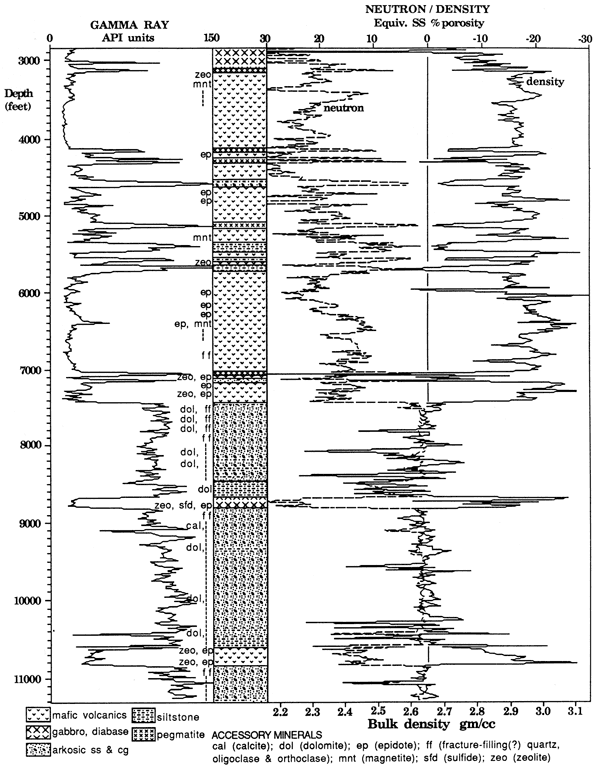
\includegraphics [keepaspectratio,width = 4.7cm] {lithologyGamma.png}
%\caption{default}
%\label{default}
\end{center}
\end{figure}
\end{column}
\end{columns}
\end{frame}

\begin{frame} \frametitle{Our Ideas} 
\vspace{-1cm}

\begin{columns}[onlytextwidth]
\begin{column}{0.6\textwidth}

\begin{itemize}
\item<1-> Automatic formation detection at the LWD tool:
\begin{itemize}
\item<2-> Use Lithology chart from planning as a prior 
\item<3-> Detect changes in LWD data 
\item<4-> Detect the most likely lithology chart above the LWD tool
\end{itemize}

\item<5-> Automatic formation detection at the bit:
\begin{itemize}
\item<6-> Use the updated lithology chart as a prior
\item<7-> Detect \emph{changes} in drilling parameters
\item<8-> Decide what is the most likely lithology chart above the bit
\end{itemize}
\end{itemize}
 \end{column}

\begin{column}{0.4\textwidth}

\only<2>{
\begin{figure}
\begin{center}
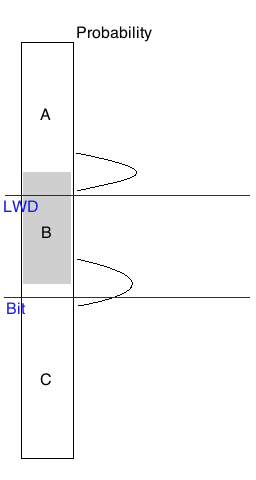
\includegraphics [keepaspectratio,width = 3.45cm] {fig2.png}\end{center}
\end{figure}
}

\only<3>{
\begin{figure}
\begin{center}
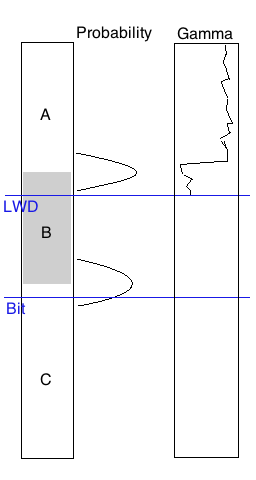
\includegraphics [keepaspectratio,width = 3.45cm] {fig3.png}\end{center}
\end{figure}
}

\only<4>{
\begin{figure}
\begin{center}
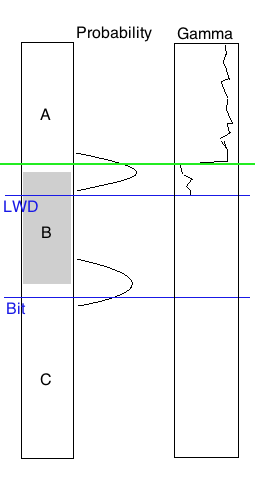
\includegraphics [keepaspectratio,width = 3.45cm] {fig4.png}\end{center}
\end{figure}
}

\only<6>{
\begin{figure}
\begin{center}
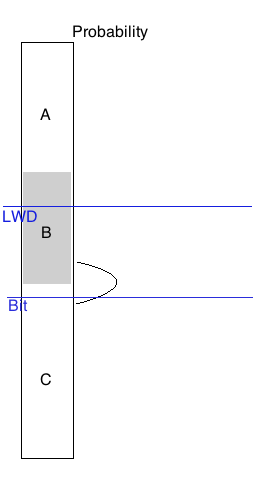
\includegraphics [keepaspectratio,width = 3.45cm] {fig5.png}\end{center}
\end{figure}
}

\only<7>{
\begin{figure}
\begin{center}
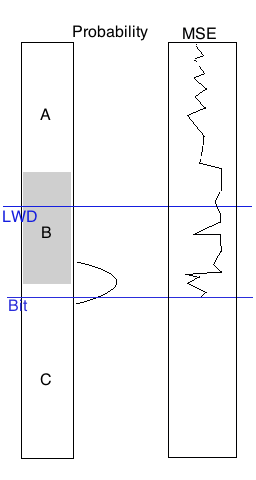
\includegraphics [keepaspectratio,width = 3.45cm] {fig6.png}\end{center}
\end{figure}
}

\only<8>{
\begin{figure}
\begin{center}
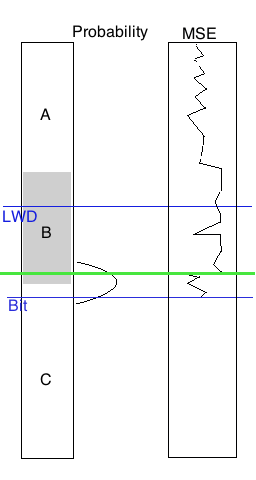
\includegraphics [keepaspectratio,width = 3.45cm] {fig7.png}\end{center}
\end{figure}
}

\end{column}
\end{columns}

\end{frame}


\begin{frame} \frametitle{How to use Information From Offset Data?} 
\vspace{-1cm}

\begin{itemize}
\item<1-> Investigate formation changes on offset data:
\item<2-> How is data from formation A different from data from formation B?
\item<3-> Some easy wins:
\begin{itemize}
\item<4-> Some changes involve a clear step in MSE or a clear drilling break
\item<5-> Some changes involve a more variable MSE (interbedded formations)
\item<6-> Some changes involve ECD increase 
\end{itemize}
\item<7-> And there are data diven approaches...
\end{itemize}
\end{frame}

\begin{frame} \frametitle{Data Driven Approach to Formation Detection} 
\vspace{-1cm}

\begin{columns}[onlytextwidth]
\begin{column}{0.4\textwidth}

\begin{itemize}
\item<2-> Classification problem
\item<5-> Data is time series
\item<6-> Data is control response pairs 
\begin{itemize}
\item<6-> Flow -> pressure
\item<6-> RPM -> torque
\item<6-> WOB,RPM,flow -> ROP
\end{itemize}
\item<7-> Solution:Dynamic Bayesian networks (Kalman filters)
\end{itemize}
 \end{column}

\begin{column}{0.6\textwidth}

\only<2>{
\begin{figure}
\begin{center}
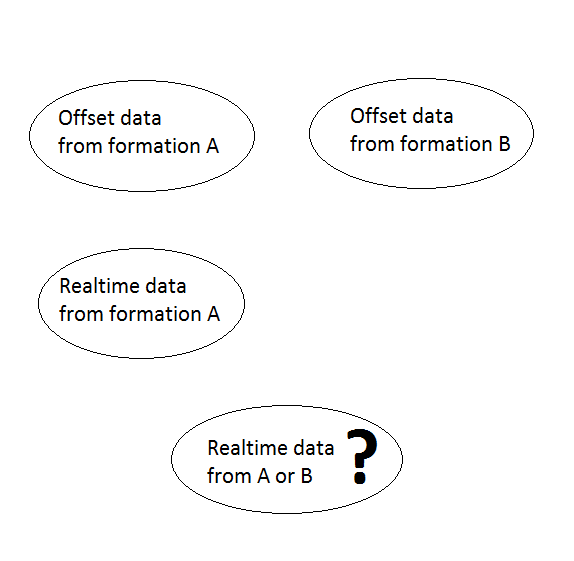
\includegraphics [keepaspectratio,width = 6cm] {figClass1.png}\end{center}
\end{figure}
}

\only<3>{
\begin{figure}
\begin{center}
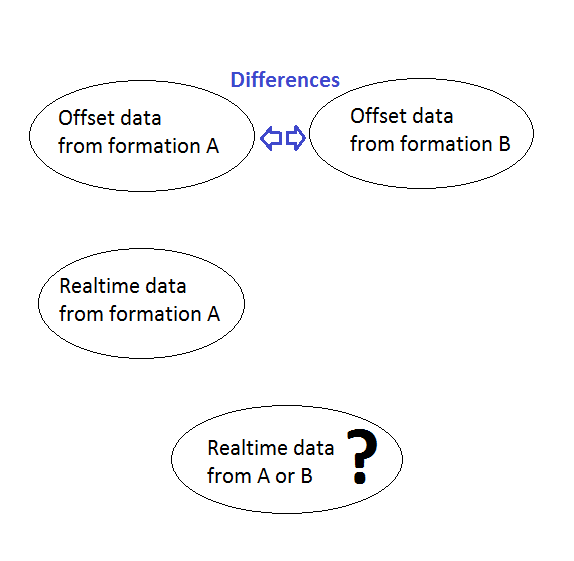
\includegraphics [keepaspectratio,width = 6cm] {figClass2.png}\end{center}
\end{figure}
}

\only<4>{
\begin{figure}
\begin{center}
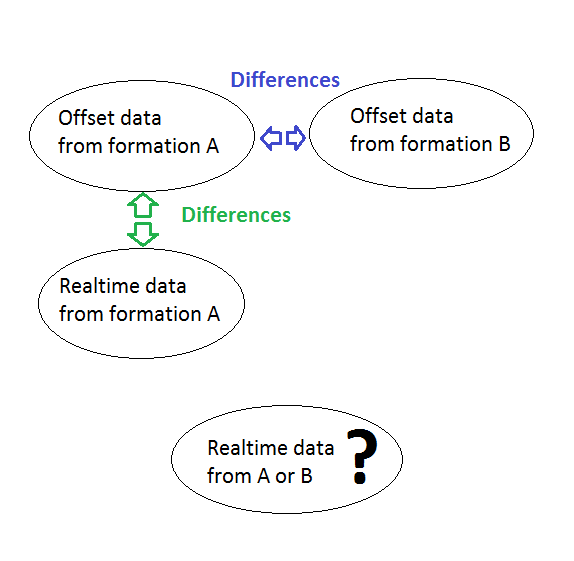
\includegraphics [keepaspectratio,width = 6cm] {figClass3.png}\end{center}
\end{figure}
}

\only<5>{
\begin{figure}
\begin{center}
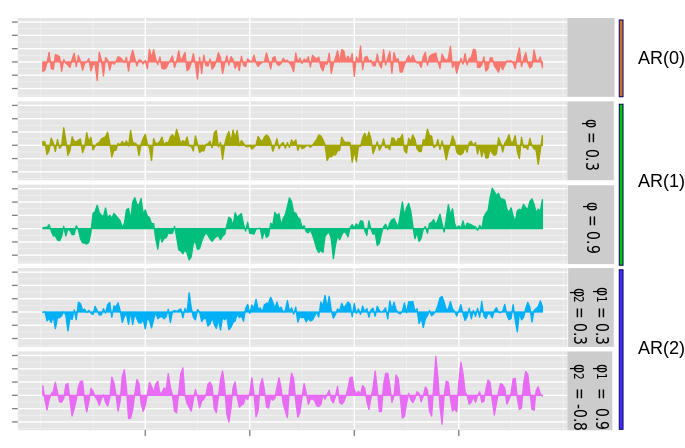
\includegraphics [keepaspectratio,width = 7cm] {ar.png}\end{center}
\end{figure}
}

\only<6>{
\begin{figure}
\begin{center}
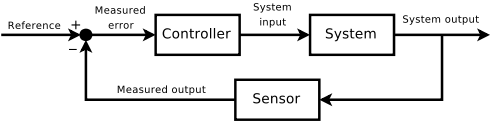
\includegraphics [keepaspectratio,width = 7cm] {control.png}\end{center}
\end{figure}
}


\only<7>{
\begin{figure}
\begin{center}
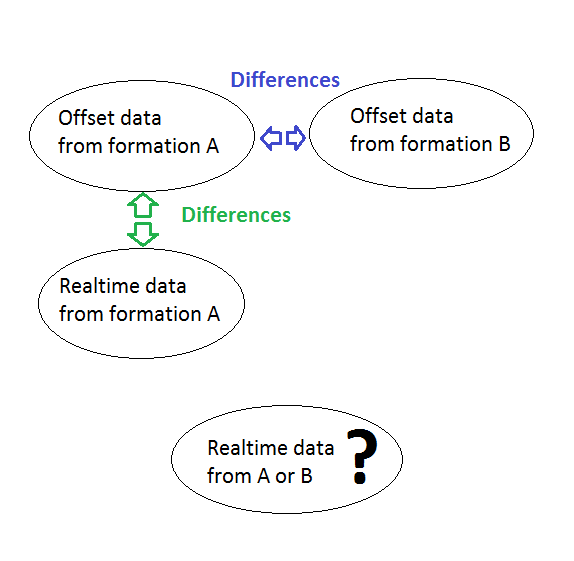
\includegraphics [keepaspectratio,width = 6cm] {figClass3.png}\end{center}
\end{figure}
}

\only<8>{
\begin{figure}
\begin{center}
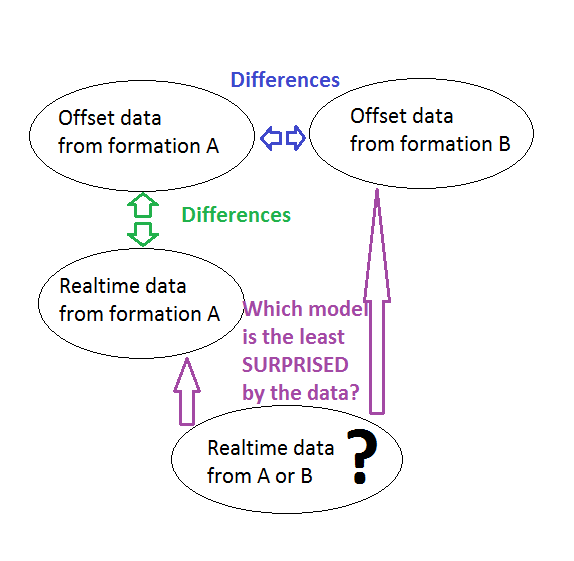
\includegraphics [keepaspectratio,width = 6cm] {figClass4.png}\end{center}
\end{figure}
}

\end{column}
\end{columns}

\end{frame}




\begin{frame} \frametitle{Mechanical Specific Energy MSE} 
\vspace{-1cm}

\begin{itemize}
\item<1-> Definition:
\begin{equation*}
MSE = \frac{WOB}{A} + \frac{TRQ \times RPM}{A \times ROP} \quad \mbox{(in SI units)}
\end{equation*}
\item<1-> MSE is a measure of compression strength of the formation, but also how effective the drilling operation is.

\item<2-> Challenges with this measure:
\begin{itemize}
\item<2-> What is downhole torque? Estimate from surface or differential pressure?
\item<2-> Drifting of WOB. When is it calibrated?
\item<2-> How much to average parameters before calculation? Average on depth
\end{itemize}

\end{itemize}

\end{frame}



%---------------------------------------------------------------------------------------------

%%%%%%%%%%%%%%%%%%%%%%%%%%%%%%%%%%%%
\section{How can we Collaborate?}
%%%%%%%%%%%%%%%%%%%%%%%%%%%%%%%%%%%%

%---------------------------------------------------------------------------------------------
\begin{frame} \frametitle{How OMV can Contribute?} 
\vspace{-1cm}

\begin{itemize}
\item<1-> Drilling data (with confidentiality agreements), consisting of
\begin{itemize}
\item<1-> Surface data
\item<1-> Lithology data (before and after)
\item<1-> LWD data
\item<1-> Offset data, interpretations of offset data
\item<2-> Memory data
\item<2-> Wireline data 
\end{itemize}
\item<3-> Resource investments:
\begin{itemize}
\item<3->  Assemble data
\item<3-> Basic support in terms of interpretations
\end{itemize}
\end{itemize}

\end{frame}

\begin{frame} \frametitle{What OMV gets back?} 
\vspace{-1cm}

\begin{itemize}
\item<1-> Results from AMIDST project
\begin{itemize}
\item<1-> Academic papers 
\item<1-> Open source software code
\item<1-> The Amidst handbook
\end{itemize}
\item<2-> Knowledge gain:
\begin{itemize}
\item<2-> What is the state of art in pattern recognition on drilling data?
\item<2-> How good can we automatically predict formations at the bit and at the LWD tool?
\item<2-> Possibly more knowledge on MSE
\end{itemize}
\end{itemize}

\end{frame}


%---------------------------------------------------------------------------------------------


%---------------------------------------------------------------------------------------------
\begin{frame} \frametitle{} 
{\it This project has received funding from the European Union's Seventh Framework Program for research, technological development and demonstration under grant agreement no 619209}
\end{frame}
%---------------------------------------------------------------------------------------------

\end{document}